% Mock-up: dataset splits. Bars are to scale (1k samples = 0.16 cm).
% Split logic: neurosnn/_data/get_data.py::_partition_indices.
\documentclass[10pt]{article}
\usepackage[margin=2cm]{geometry}   % preview only
\usepackage{tikz}
\usetikzlibrary{calc}
\begin{document}

\begin{figure}[h]
\centering
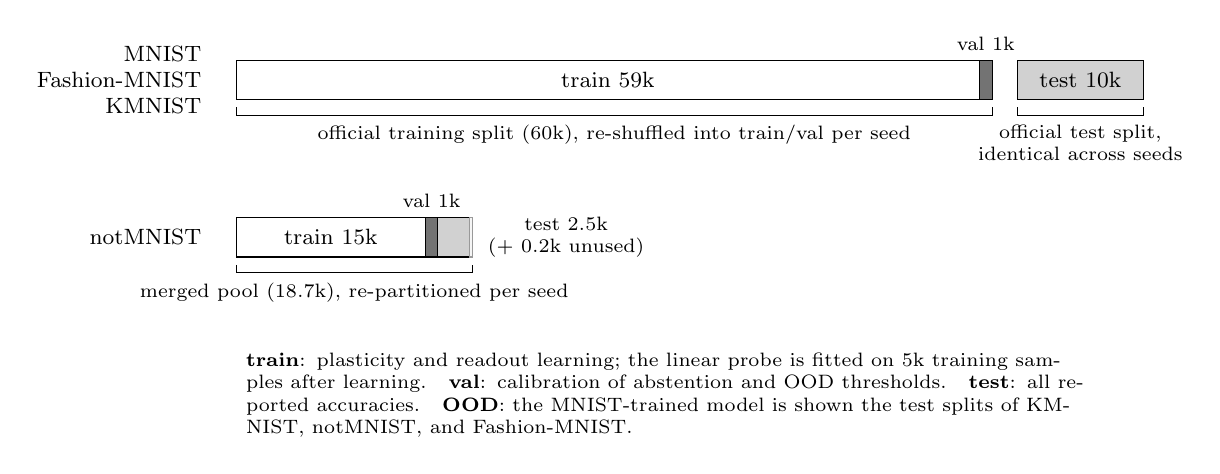
\begin{tikzpicture}[font=\footnotesize, x=0.16cm]
\tikzset{
  tr/.style={draw, fill=white},
  va/.style={draw, fill=black!55},
  te/.style={draw, fill=black!18},
  brk/.style={thin},
  lab/.style={font=\scriptsize, align=center}}

% ---------------- MNIST, Fashion-MNIST, KMNIST: dedicated test split ----------------
\node[anchor=east, align=right] at (-2,0.25) {MNIST\\Fashion-MNIST\\KMNIST};
\draw[tr] (0,0)  rectangle (59,0.5) node[midway] {train $59$k};
\draw[va] (59,0) rectangle (60,0.5);
\node[lab, above] at (59.5,0.5) {val $1$k};
\draw[te] (62,0) rectangle (72,0.5) node[midway] {test $10$k};

\draw[brk] (0,-0.1) -- (0,-0.2) -- (60,-0.2) -- (60,-0.1);
\node[lab, below] at (30,-0.2) {official training split ($60$k), re-shuffled into train/val per seed};
\draw[brk] (62,-0.1) -- (62,-0.2) -- (72,-0.2) -- (72,-0.1);
\node[lab, below] at (67,-0.2) {official test split,\\identical across seeds};

% ---------------- notMNIST: no published split, merged pool ----------------
\node[anchor=east] at (-2,-1.75) {notMNIST};
\draw[tr] (0,-2)    rectangle (15,-1.5) node[midway] {train $15$k};
\draw[va] (15,-2)   rectangle (16,-1.5);
\draw[te] (16,-2)   rectangle (18.5,-1.5);
\draw[draw=black!40, fill=black!4] (18.5,-2) rectangle (18.72,-1.5);
\node[lab, above] at (15.5,-1.5) {val $1$k};
\node[lab, right] at (19.2,-1.75) {test $2.5$k\\(+ $0.2$k unused)};

\draw[brk] (0,-2.1) -- (0,-2.2) -- (18.72,-2.2) -- (18.72,-2.1);
\node[lab, below] at (9.36,-2.2) {merged pool ($18.7$k), re-partitioned per seed};

% ---------------- what each split is used for ----------------
\node[anchor=north west, lab, align=left, text width=11cm] at (0,-3.1) {%
  \textbf{train}: plasticity and readout learning; the linear probe is fitted on
  $5$k training samples after learning.\quad
  \textbf{val}: calibration of abstention and OOD thresholds.\quad
  \textbf{test}: all reported accuracies.\quad
  \textbf{OOD}: the MNIST-trained model is shown the test splits of KMNIST, notMNIST,
  and Fashion-MNIST.};
\end{tikzpicture}
\caption{Data splits, drawn to scale. For the MNIST family, training and validation
samples are drawn from the official training split and the official test split is used
unchanged, so the test set is the same for every seed. notMNIST has no published split,
so its images are pooled and partitioned anew for each seed.}
\label{fig:data_splits}
\end{figure}

\end{document}
